%! Aldo Luna, Alexandra Mazzetti, Carlos Aznarán, Edward Canales
%! Universidad Nacional de Ingeniería
%! Facultad de Ciencias
%! Lima, Perú
%! Uso:
%! $ sudo pacman -Syu texlive-most zathura # dependencias, visor
%! $ arara solution_tercera
%! $ zathura solution_tercera.pdf
%! Ver https://wiki.archlinux.org/title/TeX_Live
% arara: clean: {
% arara: --> extensions:
% arara: --> ['aux','log','nav',
% arara: --> 'out','snm','toc','pytxcode','pdf']
% arara: --> }
% arara: lualatex: {
% arara: --> shell: yes,
% arara: --> draft: yes,
% arara: --> interaction: batchmode
% arara: --> }
%! arara: biber
%! arara: pythontex
% arara: lualatex: {
% arara: --> shell: yes,
% arara: --> draft: yes,
% arara: --> interaction: batchmode
% arara: --> }
% arara: lualatex: {
% arara: --> shell: yes,
% arara: --> synctex: yes,
% arara: --> interaction: batchmode
% arara: --> }
% arara: clean: {
% arara: --> extensions:
% arara: --> ['aux','log','nav',
% arara: --> 'out','snm','toc','pytxcode']
% arara: --> }
\PassOptionsToPackage{svgnames}{xcolor}
\documentclass[
	spanish,
	8pt,
	utf8,
	xcolor=table,
	handout,
	aspectratio=169,
	professionalfonts,
	% notheorems,
	mathserif,
	leqno,
	% t
]{beamer}
\setbeamersize{text margin left=5pt,text margin right=5pt}
\usepackage[spanish,es-sloppy]{babel}
\spanishdatedel\decimalpoint
\usepackage{mathtools}
\usepackage{nicematrix}
\usepackage{systeme}
\usepackage{minted}
\usepackage{enumerate}
\usepackage{multicol}
% \usepackage{pythontex}
\usepackage[
	citestyle=numeric,
	style=apa,
	backend=biber,
	defernumbers=true,
	sorting=ynt,
	maxcitenames=4
]{biblatex}
\addbibresource{references.bib}

\newcolumntype{x}[1]{>{\centering\arraybackslash\hspace{0pt}}p{#1}}

\newcounter{savedenum}
\newcommand*{\saveenum}{\setcounter{savedenum}{\theenumi}}
\newcommand*{\resume}{\setcounter{enumi}{\thesavedenum}}

\setbeamertemplate{navigation symbols}{}
\setbeamertemplate{footline}{}
\setbeamertemplate{headline}{}

% https://tex.stackexchange.com/questions/68080/beamer-bibliography-icon
\setbeamertemplate{bibliography item}{%
	\ifboolexpr{ test {\ifentrytype{book}} or test {\ifentrytype{mvbook}}
		or test {\ifentrytype{collection}} or test {\ifentrytype{mvcollection}}
		or test {\ifentrytype{reference}} or test {\ifentrytype{mvreference}} }
	{\setbeamertemplate{bibliography item}[book]}
	{\ifentrytype{online}
		{\setbeamertemplate{bibliography item}[online]}
		{\setbeamertemplate{bibliography item}[article]}}%
	\usebeamertemplate{bibliography item}}

\defbibenvironment{bibliography}
{\list{}
	{\settowidth{\labelwidth}{\usebeamertemplate{bibliography item}}%
		\setlength{\leftmargin}{\labelwidth}%
		\setlength{\labelsep}{\biblabelsep}%
		\addtolength{\leftmargin}{\labelsep}%
		\setlength{\itemsep}{\bibitemsep}%
		\setlength{\parsep}{\bibparsep}}}
{\endlist}
{\item}

\makeatletter
\newenvironment<>{proofs}[1][\proofname]{%
    \par
    \def\insertproofname{#1\@addpunct{.}}%
    \usebeamertemplate{proof begin}#2}
  {\usebeamertemplate{proof end}}
\makeatother


\title{
	\huge\sffamily
	Práctica Dirigida
}

\subtitle{
	\large\scshape
	Análisis y Modelamiento Numérico I\quad CM4F1 B\\[.5\baselineskip]
		\normalsize\normalfont
		Profesor Ángel Enrique Ramírez Gutiérrez.
}

\author{
	Carlos A. Aznarán Laos
}

\institute{\large
	Facultad de Ciencias \and
	Universidad Nacional de Ingeniería
}
\date{\today}

\begin{document}

\frame{\titlepage}

\begin{frame}

	\begin{enumerate}%\setcounter{enumi}{0}
		\item

		      Calcule la solución de mínimos cuadrados del sistema $Ax=b$
		      donde:
		      \begin{equation*}
			      A=
			      \begin{bNiceMatrix}
				      1 & -6 \\
				      1 & -2 \\
				      1 & 1  \\
				      1 & 7
			      \end{bNiceMatrix},\quad
			      b =
			      \begin{bNiceMatrix}
				      -1 \\
				      2  \\
				      1  \\
				      6
			      \end{bNiceMatrix}.
		      \end{equation*}
		      \saveenum
	\end{enumerate}

	\begin{solution}
		$$
			A^{\top} A=\left(\begin{array}{cccc}
					1  & 1  & 1 & 1 \\
					-6 & -2 & 1 & 7
				\end{array}\right)\left(\begin{array}{cc}
					1 & -6 \\
					1 & -2 \\
					1 & 1  \\
					1 & 7
				\end{array}\right)=\left(\begin{array}{cc}
				4          & 0 \\
				4 \times 2 & 0
			\end{array}\right)_{2 \times 2}
		$$
		$\left(A^{\top} A\right)^{-1}=\left(\begin{array}{cc}1 / 4 & 0 \\ 0 & 1 / 90\end{array}\right)$

		$x=\left(A^{\top} A\right)^{-1} A^{\top} b=\left(\begin{array}{cccc}1 / 4 & 1 / 4 & 1 / 4 & 1 / 4 \\ 1 / 15 & -1 / 45 & 1 / 90 & 9 / 90\end{array}\right)\left(\begin{array}{c}-1 \\ 2 \\ 1 \\ 6\end{array}\right)_{4 \times 1}=\left(\begin{array}{c}2 \\ 1 / 2\end{array}\right)$
		% \begin{aligned}
		% 	 & \left.x=A^{\top} A\right)^{-1} A^{\top} b=\left(\begin{array}{cccc}
		% 			                                                   1 / 4  & 1 / 4   & 1 / 4  & 1 / 4  \\
		% 			                                                   1 / 15 & -1 / 45 & 1 / 40 & 7 / 40
		% 		                                                   \end{array}\right)\left(\begin{array}{l}
		% 		                                                                           -1 \\
		% 		                                                                           2  \\
		% 		                                                                           1  \\
		% 		                                                                           6
		% 	                                                                           \end{array}\right)_{4 \times 1}=\left(\begin{array}{c}
		% 			                                                                                                                 2 \\
		% 			                                                                                                                 1 / 2
		% 		                                                                                                                 \end{array}\right) \\
		% 	 & x=\left(\begin{array}{c}
		% 			           2 \\
		% 			           1 / 2
		% 		           \end{array}\right)                                                                                                       \\
		% 	 &
		% \end{aligned}
		% 		Considere el problema de encontrar un vector $x\in\mathbb{R}^{n}$
		% 		tal que $Ax=b$ donde la matriz de datos
		% 		$A\in\mathbb{R}^{n\times n}$ y el vector de observación
		% 		$b\in\mathbb{R}^{m}$ son dados y $m\geq n$.

		% 		\begin{align*}
		% 			A                            x                           & =b.                                        \\
		% 			\shortintertext{Multiplicamos a izquierda por \alert{$A^{T}$}}
		% 			\alert{A^{T}}A               x                           & =\alert{A^{T}}b.                           \\
		% 			\alert{\left(A^{T}A\right)}  x                           & =A^{T}b.                                   \\
		% 			\shortintertext{Multiplicamos a izquierda por $\alert{{\left(A^{T}A\right)}^{-1}}$}
		% 			\alert{{\left(A^{T}A\right)}^{-1}}\left(A^{T}A\right)  x & =\alert{{\left(A^{T}A\right)}^{-1}}A^{T}b. \\
		% 			\Aboxed{x                                                & ={\left(A^{T}A\right)}^{-1}A^{T}b.}
		% 		\end{align*}
	\end{solution}
\end{frame}

% \begin{frame}
% 	\begin{solution}
% 		.
% 	\end{solution}
% \end{frame}

\begin{frame}
	\begin{enumerate}
		\resume
		\item

		      Encuentre la recta que da el mejor ajuste para los datos
		      \begin{equation*}
			      \mathcal{S}=
			      % {\left\{
			      % \left(t_{i},b_{i}\right)\right\}
			      % }_{i=1}^{4}=
			      \left\{
			      \left(1,2\right),
			      \left(2,3\right),
			      \left(3,5\right),
			      \left(4,7\right)
			      \right\}.
		      \end{equation*}
		      \saveenum
	\end{enumerate}

	\begin{solution}
		Ajustaremos el conjunto de datos $\mathcal{S}$ la función $y=mx+b$.
		% $f\left(x_{0},x_{1},t\right)=x_{0}+x_{1}t$.
		\begin{table}[ht!]
			\centering
			\begin{tabular}{|c|c|c|c|}
				\hline
				$x_{i}$         & $y_{i}$         & $x_{i}y_{i}$         & $x_{i}^{2}$         \\
				\hline
				$1$             & $2$             & $1\times 2=2$        & $1^{2}=1$           \\
				$2$             & $3$             & $2\times 3=6$        & $2^{2}=4$           \\
				$3$             & $5$             & $3\times 5=15$       & $3^{2}=9$           \\
				$4$             & $7$             & $4\times 7=28$       & $4^{2}=16$          \\
				\hline
				$\sum x_{i}=10$ & $\sum y_{i}=17$ & $\sum x_{i}y_{i}=51$ & $\sum x_{i}^{2}=30$ \\
				\hline
			\end{tabular}
		\end{table}

		\begin{itemize}
			\item

			      Encontrar el valor de $m=\frac{n\sum x_{i}y_{i}-\sum x_{i}\sum y_{i}}{n\sum x_{i}^{2} - \left(\sum x_{i}\right)^{2}}$.

			\item

			      Encontrar el valor de $b=\frac{\sum y_{i}-m\sum x_{i}}{n}$
		\end{itemize}

		% Para los datos y parámetros de este ejemplo el sistema $Ax=b$
		% tiene la forma siguiente:
		% \begin{equation*}
		% 	\begin{bNiceMatrix}
		% 		1
		% 	\end{bNiceMatrix}
		% 	\begin{bNiceMatrix}
		% 		x_{0} \\
		% 		x_{1}
		% 	\end{bNiceMatrix}=
		% 	\begin{bNiceMatrix}
		% 		2 \\
		% 		3 \\
		% 		5 \\
		% 		7
		% 	\end{bNiceMatrix}
		% \end{equation*}
	\end{solution}
\end{frame}

\begin{frame}[fragile]
	\begin{minipage}{0.45\textwidth}
		\begin{figure}[ht!]
			\centering
			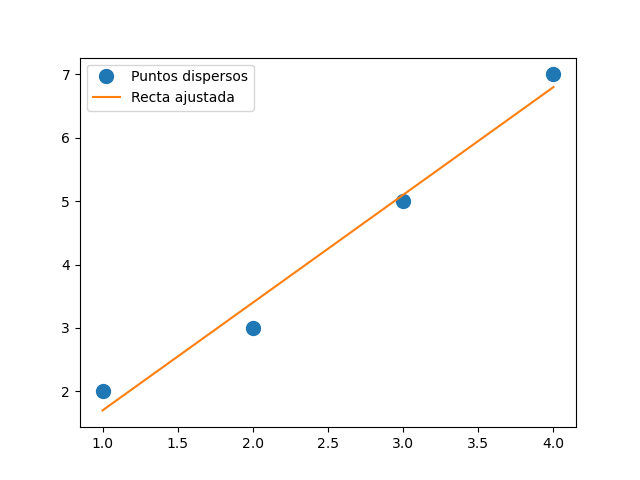
\includegraphics[width=6.5cm]{fitted}
		\end{figure}
	\end{minipage}
	\begin{minipage}{0.45\textwidth}
		\begin{listing}[H]
			\inputminted[
				fontsize=\scriptsize,
				breaklines,
			]{python}{dirigida.py}
		\end{listing}
	\end{minipage}
\end{frame}

% \begin{frame}
% 	\begin{enumerate}
% 		\resume
% 		\item
% 		      Sea

% 		      \begin{equation*}
% 			      A=
% 			      \begin{pNiceMatrix}
% 				      2 & 1 \\
% 				      1 & 1 \\
% 				      2 & 1
% 			      \end{pNiceMatrix}
% 			      \text{ y }
% 			      b=
% 			      \begin{pNiceMatrix}
% 				      12 \\
% 				      6  \\
% 				      18
% 			      \end{pNiceMatrix}.
% 		      \end{equation*}

% 		      \begin{enumerate}
% 			      \item

% 			            Use el proceso de Gram-Schmidt para determinar una
% 			            base ortonormal para el espacio columna de $A$.

% 			      \item

% 			            Factorice $A$ en un producto $Q R$ donde $Q$ es un
% 			            conjunto ortogonal de vectores columna es
% 			            triangular superior.

% 			      \item

% 			            Resuelva el problema de mínimos cuadrados.

% 		      \end{enumerate}

% 		      \saveenum
% 	\end{enumerate}

% 	\begin{solution}
% 		.
% 	\end{solution}
% \end{frame}

% \begin{frame}
% 	.
% \end{frame}
\end{document}